\chapter{市场调查与分析}

\section{亲子主题餐饮产业链分析}
基于传统餐饮行业的产业链来看,上游行业是食品开发、生产和物流配送、厨师培
训;由于亲子主题餐饮的特殊性,还涉及到幼教培训机构,装修公司,室内设计行业。
终端消费者就是中等收入人群及其子女。其产业链条如图~\ref{figure:inds-chain}所示。
\begin{figure}
        \centering
        \caption{产业链}
        \label{figure:inds-chain}
        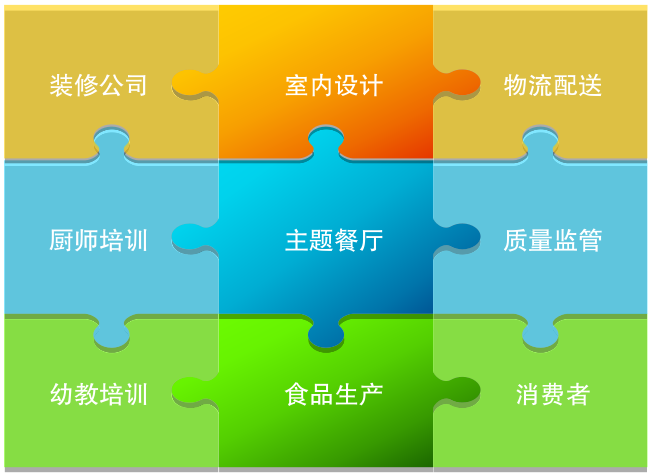
\includegraphics[ width=\textwidth ]{../images/company/inds-chain}
\end{figure}

\paragraph{食品生产}
对餐饮业而言,食品安全是企业良性发展的基石。尤其是在各种食品安全事件已成
为百姓心中挥之不去的阴霾的当下,餐饮企业对食品安全的重视程度和把控能力更成为
消费者信心的风向标。为此,公司全力确保食品生成企业的安全可靠,对不同的食品供
应商进行等级评分机制;设立专门的食品检验部门,把检验出问题的食品供应商列入黑
名单。

\paragraph{室内设计}
用餐环境和室内设计有着密不可分的关系。公司的目标是设计温馨舒适、时尚高雅
的用餐环境。为此,我们选用国内知名装修公司进行室内的装修,努力为消费者打造视
觉的享受,为每一个细节铸就一丝不苟的印象。

\paragraph{物流配送}
运输不仅是物流的重要职能之一,同时运输贯穿于产品的整个流通过程之中,从原材
料采购到产品分销这一过程中,各个节点之间物质实体的联系也是运输,运输不仅横贯了
企业的各职能部门,而且越过了企业的边界将上游和下游的企业联结起来。我们使用顺丰
作为物流公司。

\paragraph{厨师培训}
厨师是菜品的制作者,关乎出品的好坏。我们从知名职业学校的烹饪专业招聘熟练
的厨工,从行业上高薪聘请有丰富经验的大厨来确保每一道菜的质量。从海外高等院校
的营养学专业聘请膳食专作为食品营养方面的咨询。

\paragraph{装修公司}
\subparagraph{精简为主,拒绝豪华}
可能很多人会认为,餐厅装修的越豪华就越会吸引到更多的
顾客。有些小餐馆在装修前,总想着将自己的店铺设计的豪华靓丽、高端大气上档次,
以为这样就会使自己的餐馆更有竞争力,其实不然。一般小餐饮店的消费者都是以工薪
群体为主的,他们的消费水平并不会太高。如果他们看到餐厅装修得特别豪华,可能不
会选择走进去,因为在他们心里这种餐厅菜价都很高。从这方面来考虑,小餐饮店的装
修并非越豪华越好,它必须结合当地的收入水平以及餐饮店所在位置周围的消费群体来
确定风格及档次。如果要选择设计公司,应该是那些对小餐饮店装修比较有经验的来进
行装修设计。
\subparagraph{ 前厅宽敞,拒绝拥挤 }
小餐饮店一般客流量比较大,所以餐厅的前厅应该设计的宽
敞、明亮,其高度应不低于 3 米。经营不同风味菜品对其前厅面积的要求也有所不同,
比如经营烤鸭、家常菜的餐馆,由于菜品丰富、上菜程序复杂、客流量大,设计这样的
前厅面积最小不应少于 400 平方米。否则顾客多,就餐面积过小,会使顾客感到杂乱无
章,影响就餐的心情。同时,在混乱环境中工作的服务员也会感到手忙脚乱易出事故。
\subparagraph{ 注重背景墙,色调要适宜 }
现在的餐厅不再是以前那种简单的白色墙面,经营者善
于利用背景墙来表现餐厅的特色很关键。背景墙不仅能营造温馨的用餐氛围,还有助于
提升整个房子的格调。至于背景墙要选择什么色调,这个要根据餐厅的空间大小来决定。
若餐厅空间较小则可以采用淡色调来扩大空间感;若餐厅空间很大则可以以重色为主,
淡色为辅,达到沉稳却不沉闷的效果。

\paragraph{幼教培训}
由于我们的主要客户是儿童,我们必须为有学前教育资格的服务人员提供娱乐。在
蛋糕 DIY 等一些儿童活动中,我们还要求服务人员具有学前教育和烹饪的双重资格。具
体而言,我们需要以下资质和能力:

\subparagraph{ 了解心理学 }
儿童之间的个体差异非常大(有些儿童在 4 岁时具有 5 岁的发育特征,
并且有些儿童在 4 岁时仍然保持在 3 岁)。只有具备心理学知识,我们才能分析孩子的
方面。发展更好,需要更多关注。

\subparagraph{ 愿意学习,勇于尝试,善于总结 }
做更多的专业培训。除了不断更新知识,儿童不
会面临相同的环境刺激,每一代都是不同的。例如,现今的孩子喜欢玩平板电脑等电子
设备,这对他们的耐心,专注和想象力产生很大的负面影响。
个性比较好。个性好的范围并不局限于传统的亲和力概念。从小孩到父母到同事到
路人,能够与任何人成为朋友。不难理解,与孩子交朋友是一项专业要求。成为父母的
朋友,保持专业素质。在与父母谈论孩子的情况时,婉转表达孩子面临的问题。与同事
的关系也要好,因为孩子会在无意识中模仿和学习,如果你与同事冷淡交谈,可以想象
对孩子的负面影响。

\subparagraph{ 保持专业 }
不能将孩子的照片发送到社交媒体,如朋友圈和微博。也不可能接受父
母的礼物,接受父母的饭食,并且与工作以外的父母建立关系。对于出现在新闻中的打
鼾儿童,这更令人无法接受。

\subparagraph{ 知识结构和视角 }
除了尽可能多地了解诗歌和绘画外,知识结构和视野也非常重要。
因为儿童餐馆在小学和中学所学的东西不同,中小学都是学科。我们亲子活动的目的是
教育孩子学习如何生活并理解生活中的世界。

\paragraph{消费者}
我们面向社会开展营业,目标用户是带小孩的家长,年轻孕妇和二胎孕妇,3--12 周
岁的儿童;一般社会人士。

\section{竞争因素分析}
\subsection{竞争产品分析}
餐饮行业已经是一个成熟的行业,有许多国内外大品牌,如百胜餐饮旗下的肯德基、
必胜客,中国本土的李先生、蒸功夫,还有一些城市的本地品牌,在当地颇具影响力。
这些传统餐饮行业的佼佼者就是我们最为直接有力的竞争者。它们拥有可观的客户群,
财力雄厚,有着完整的供应链条,成熟的经验模式和丰富的运作经验。

目前,亲子主题餐饮的主要替代品是其他一些能够满足亲子需要的餐饮,比如孩子
普遍喜欢的洋快餐和父母喜欢的中餐馆等。我们要抓住健康这个话题,利用父母关系孩
子的饮食健康和营养的心理,提供健康美味,营养丰富的食品。为了能够满足孩子们猎
奇的心理,我们的菜式要多种多样,不断创新,不落俗套,这样才能吸引孩子的眼球。
从家长的角度考虑,我们要提供亲子交互的平台和机会,例如一些益智游戏,DIY 活动
等等;活动以健康有益,促进亲子关系为出发点,不断推出新花样,保持家长和孩子的
新鲜感。

互联网营销建立在互联网上,所以企业可以选择拥有更多优势网站来建立自己的网
站,然后专门进行维护管理,这样可以节省传统营销的很多广告费用,搜索引擎也会关
注搜索率网站。

传统餐饮行业非常注重食品安全,稍微高档一点的餐厅会重视服务员的服务态度和
装修装潢。为了能与它们竞争,我们要采用更加严格的食品安全保障措施,确保出品的
质量;我们的服务员要有像幼儿园老师一样的耐心对待孩子,态度热情大方;组织亲子
活动的服务人员要熟悉幼儿心理,在游戏活动中让孩子收获快乐,成长和友情,让家长
陪伴孩子度过一段快乐的,有意义的时光。这是我们与传统餐饮行业的最大区别。

\subsection{潜在进入者分析}
% TODO Fix this broken table
\begin{table}[ htbp ]
\caption{潜在进入者}
\centering
\begin{tabular}{|c|c|c|p{5cm}|}
\hline
       公司名称        &       地址            &                菜系或特色\\
\hline
北京麦幼优儿童主题餐厅 &海淀区北三环西路 23 号中坤广场 D 座 3 楼(近大钟寺地铁站) 
&西餐、甜品饮品、休闲家庭套 餐为主\\
\hline
上海芭迪熊儿童主题餐厅 &长宁区长宁路 1018 号龙之梦购物中心&蘑菇房餐厅\\
\hline
广州熊猫餐厅&广州番禺迎宾路&餐厅共有 600 多个餐位,
提供川菜、广东本地美食,还有日本以及越南、新加坡、泰国等东南亚美食,味道地道正宗。\\
\hline
\end{tabular}
\end{table}




\begin{figure}[htbp]
        \caption{北京麦幼优儿童主题餐厅}
        \centering
        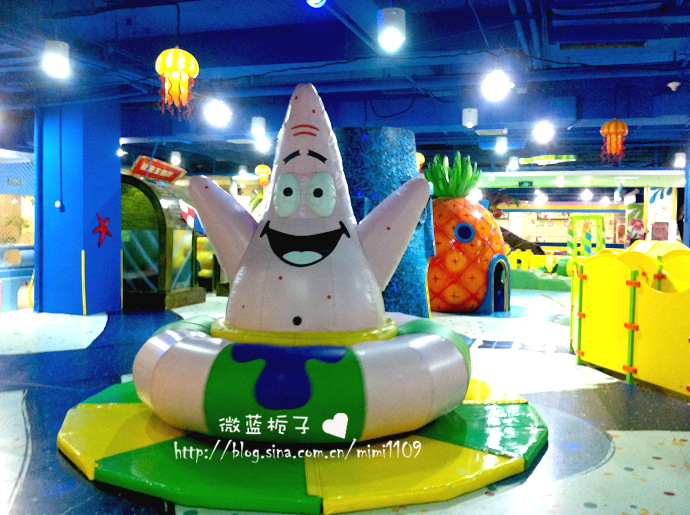
\includegraphics[width=0.6\textwidth]{../images/competitors/北京麦幼优儿童主题餐厅}
\end{figure}

% Note the percetage %, without them 2 subfigures will be vertically placed.
% Using %, the newline is suppressed.
% The effect is not as good. Uses subcaption and caption packages.
\begin{figure}[htbp]
        \begin{subfigure}[b]{0.5\textwidth}
                \caption{上海芭迪熊儿童主题餐厅}
                \centering
                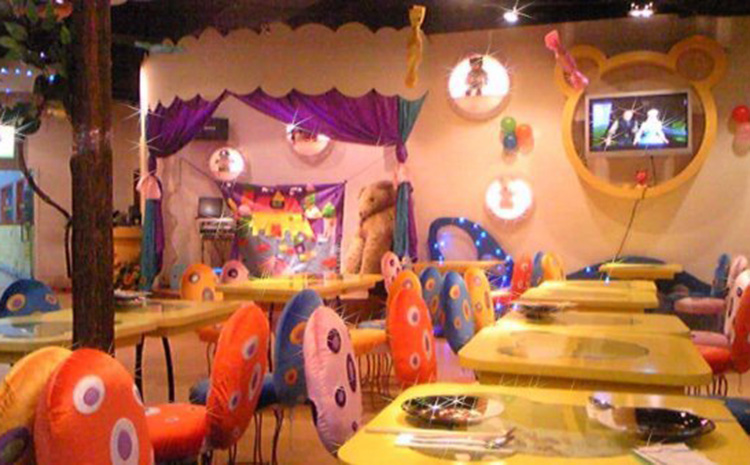
\includegraphics[width=0.6\textwidth]{../images/competitors/上海芭迪熊儿童主题餐厅}
        \end{subfigure}%
%
        \begin{subfigure}[b]{0.5\textwidth}
                \caption{广州熊猫餐厅}
                \centering
                % How to scale image to the same width as text block
                % https://tex.stackexchange.com/questions/39147/scale-image-to-page-width
                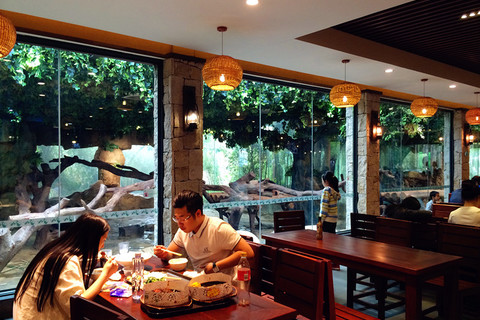
\includegraphics[width=0.6\textwidth]{../images/competitors/广州熊猫餐厅}
        \end{subfigure}%
\end{figure}

\paragraph{北京麦幼优儿童主题餐厅}
马来西亚著名 STATIONONE 餐饮集团与北京麦幼优投资有限公司共同投资的国内首
家麦幼优儿童主题餐厅旗舰店,整个主题餐厅近 300 平米,装修风格为东南亚热带雨林
特色,菜品主要以休闲西餐、甜品饮品、以及休闲家庭套餐为主,兼顾餐饮、娱乐与教
育三大功能。孩子和家长在这里不仅可以品尝到马来西亚美食,用餐后还可观赏有趣的
表演,参加互动活动。同时,餐厅还可以让孩子亲手制作菜品,体验“DIY 小达人”、“明
星小厨师”、“魔幻小天地”等多项活动,展示孩子的创造力和想象力。

\paragraph{上海芭迪熊儿童主题餐厅}
芭迪熊是沪上第一家属于孩子的餐厅,服务对象是 1--12 岁的儿童。与其说他是一
个餐厅,更不如说它是一个在钢筋丛林里的童话世界。蘑菇饮料站,橘红色的蘑菇顶,
碧绿的蘑菇身子,高高的绿色小蘑菇高坐椅围在大蘑菇饮料站的四周。彩色的花朵餐桌
和鲜艳的异型坐椅,分外引人注目。非常可爱的装盘,让孩子能愉快地用餐。

\paragraph{广州熊猫餐厅}
广州长隆野生动物世界打造的全球首个“与熊猫共餐”主题餐厅于 2013 年元旦开业
迎客,餐厅与生态竹林巧妙融合,最为惊喜的是,游客可在“国宝”级生态环境中,与大
名鼎鼎的熊猫“津柯”、“银柯”共进大餐。熊猫餐厅的出品也十分国际化。

\subsection{竞争优势分析}
我们的优势在于兼顾了父母和孩子的用餐体验。许多已有的亲子餐厅只是儿童化的
装修+儿童游乐设施+普通餐饮的简单结合。而我们主打的营养健康理念将别树一帜:我
们从世界各地甄选食材,请专业的营养师为每一位顾客量身打造每一顿的营养配比,这
是其它亲子餐厅无法比拟的。

此外,我们还定期举办免费的亲子出游、读书、两人三足、趣味拔河等趣味活动,
邀请会员参加。事实上,我们将竭力打造一个围绕亲子展开的多元文体活动社区,让亲
子互动不止与吃喝。

网络营销与传统营销模式的区别在于其独特的互动模式。 根据公司产品的特点,
网络营销可以根据具体的目标客户和独特的企业文化加强互动,节约开支,传统营销模
式的营销模式单一。

由于我们对服务的精益求精,我们还定期邀请孩子和家长参与我们的《美食在哪里》
活动。活动的形式为乘坐观光电扶梯参观我们食品生成的内部环节。这个活动一方面可
以向消费者公开我们的生产环境,另一方面也起到观光旅游的作用。

\section{市场发展预期走势分析}
\begin{table}[htbp]
\centering
\caption{表格 3 市场发展走势分析}
\begin{tabular}{|c|c|c|c|c|c|}
\hline
年份&2014&2014--2015&2015--2016&2016--2017&2017后\\
\hline
空间&概念年&开发年&实验年&推广年&火爆年\\
\hline
\end{tabular}
\end{table}

在现代人以父母--子女为中心的家庭关系中,维护和培养亲子关系越来越多的成为
有一定教育水平的父母的共识。在现代人忙碌快节奏的生活中,亲子餐厅就像茫茫水泥
森林中绿树成荫的一角,带给父母和孩子一片温馨愉快的绿荫。在越来越多父母重视和
孩子的精神交流的今天,亲子餐厅以其与众不同的用餐体验,正越来越受到青睐。随着
更多以亲子互动为特色的餐厅进入该行业,价格的下降将会引来更多的消费者体验这一
温馨的用餐体验。

从图表上看,亲子主题餐饮在销售总额上不及传统餐饮,这也恰恰说明这个新兴行
业具有很大的发展空间。而且近 3 年来,亲子主题餐饮都保持了一定的增速,再次说明
了它的增值潜力。

\section{市场预测分析}

\subsection{预测的市场规模和总容量}
自从国家实施二孩政策以来,我国有望迎来新一个生育大潮,这意味着我国人口老
龄化的速率将减缓,不少家庭因为二孩的出生而形成孩子小,父母老的局面。调查显示,
截至 2018 年 1 月 1 日,我国累计出生的二孩高达 2.5 千万人,这就是一个不可估量的
市场。许多二孩的父母在拥有了更好的条件之后像给孩子一个不一样的童年——他们成
为亲子餐厅的重要目标客户。

网络营销渠道必须从消费者的角度出发。 为吸引消费者购买,应及时在公司网站
上发布促销信息,新产品信息,公司动态,并开放多种支付方式,方便消费者购买建议,
以便消费者选择。 在网站上设置人工客户服务。 为了吸引消费者关注网络中的产品,
有可能扩展公司的产品。 例如,在网站的建设中,可以及时建立在线商店,增加销售
渠道。

除了二孩家庭外, 90 后的年轻一代也逐渐进入结婚生子的进程。他们大多数受过高
等教育,懂得孩子的成长离不开父母和孩子的精神交流。许多人都有着为了庆祝家里高
兴的事情而外出就餐的经历,相信有幼龄的 90 家庭会选择更加照顾孩子的餐厅——亲
子主题餐厅。调查显示,已婚的 90 后人数高达 3.2 千万人,这也是一个非常有潜力的市场。

总之, 90 后市场和二孩政策产生的二孩家庭为我们提供了广泛的市场。以每家每次
平均消费 250 元,每天一家门店招待 50 个家庭来计算,一年将产生 456 万元的营业额,
相当可观。

\subsection{行业市场划分与应用内容}
根据市场调研,目前进行亲子主题餐饮的实体主要有:
\begin{enumerate}[1)]
\item
广州长隆集团开发了熊猫酒店、海底餐厅、白虎餐厅等。
\item
中外合资的亲子餐厅。
\item
其他独立运营的民营亲子餐厅。
\end{enumerate}

\subsection{亲子主题餐饮的商业模式}
目前根据的盈利模式主要有三种:
\begin{enumerate}[1)]
\item
直接消费模式: 顾客来到餐馆就餐,然后收取相应的费用。
\item
亲子互动服务模式: 顾客来到餐馆,进行各种亲子互动活动,收取相应的费用。
\item
捆绑旅游项目模式: 餐馆把上述两种盈利方式打包,作为其他旅游项目的一部分,
旅客通过旅行社间接支付费用。
\end{enumerate}
